\documentclass{beamer}
\usetheme{Madrid}
\usepackage[utf8]{inputenc}
\usetheme{Antibes}
\usepackage{hyperref}
\usepackage{minted}
\usepackage{array}
\usepackage{graphicx}
\usepackage{algpseudocode}
\usepackage{algorithm}% 
\usepackage{multicol}
\usepackage[font=small,labelfont=bf]{caption}
\usepackage[subrefformat=parens]{subcaption}
\usepackage{comment}

\algnewcommand\And{\textbf{and}}
\algnewcommand\Or{\textbf{or}}


\definecolor{MFNGreen}{RGB}{0,124,88}

\setbeamercolor*{structure}{bg=MFNGreen!20,fg=MFNGreen}

\setbeamercolor*{palette primary}{use=structure,fg=white,bg=structure.fg}
\setbeamercolor*{palette secondary}{use=structure,fg=white,bg=structure.fg!75}
\setbeamercolor*{palette tertiary}{use=structure,fg=white,bg=black}
\setbeamercolor*{palette quaternary}{fg=white,bg=black}

\setbeamercolor{section in toc}{fg=black,bg=white}
\setbeamercolor{alerted text}{use=structure,fg=structure.fg!50!black!80!black}

\setbeamercolor{titlelike}{parent=palette primary,fg=structure.fg!50!black}
\setbeamercolor{frametitle}{bg=MFNGreen!85,fg=white}

\setbeamercolor*{titlelike}{parent=palette primary}


\setbeamertemplate{navigation symbols}{}
\setbeamertemplate{headline}{}

\title[Data Protection and Privacy]{Anonymizing transaction databases for publication: (h,k,p)-coherence}
\subtitle{Data Protection and Privacy final assignment}

\author[]{Marco Zucca
        \and 
        Chiara Cossu}

\institute[UniGe]{Università degli studi di Genova \\ Computer Science}

\date{January 2023}
\begin{document}

\maketitle

%--

%--
\begin{frame}[fragile]
\frametitle{Introduction}
What is hkp-coherence?
\begin{itemize}
    \item Anonymizing algorithm for transactional data
    \item Used for anonymizing databases for publication
    \item `` Our scenario requires publishing
sensitive information, but hiding the identity of data subjects ''
    \item ``we model
attackers’ prior knowledge as subsets of public items.''
\end{itemize}
\end{frame}
%--
\begin{frame}[fragile]
\frametitle{Glossary}
\begin{itemize}
    \item \textbf{P}: ``Power of the attacker''
    \item \textbf{$\beta$}: Set of items (public or not)
    \item \textbf{$\beta$-cohort}: Set of all transactions containing beta
    \item \textbf{H}: Percentage of private items for a $\beta$-cohort (?)
    \item \textbf{K}: Similar to the K in \textit{k-anonimity}
    \item \textbf{Sup} (=Support): Number of transactions for a $\beta$-cohort
    \item \textbf{P-breach}: The max \texttt{sup(p)} among all p restricted to a $\beta$-cohort 
    \item \textbf{Mole}: $\beta$ such that $sup(\beta) < K \lor P_{breach} > H$
    \item $\delta$: Percentage of public items
    \item \textbf{MM(e)}: The number of moles that contains $e$
    \item \textbf{IL(e)}: Information loss by removing $e$ from D
\end{itemize}
\end{frame}
%--
\begin{frame}[fragile]
\frametitle{Main algorithm: simple overview}
\begin{algorithm}[H]
\caption{Anonymization overview}\label{alg:cap}
\begin{algorithmic}
    \State{suppress all size-1 moles from D}
    \State{find moles of size in $[2,p]$
    \State{build the mole tree and its score table}
    \While{there are minimal moles in D }\State{suppress the public item e with the maximum MM(e)/IL(e) from D} \EndWhile
\end{algorithmic}
\end{algorithm}
\end{frame}
%--
\begin{frame}[fragile]
\frametitle{Implementation and features}
    \begin{itemize}
        \item Written in Python 3.9
        \item Extensive use of Pandas data structures like \texttt{DataFrames}
        \item 2 main blocks: \verb!hkp_anon.py! and \verb!mole_tree.py!
        \item takes as input a sparse matrix of 1s and 0s
        \item we tried to stick to paper implementation as much as possible
        \item additional data manipulation utilities:
        \begin{itemize}
            \item preprocessing
            \item synthetic data generator
            \item density evaluation
        \end{itemize}
    \end{itemize}
    
\end{frame}
%--
\begin{frame}[fragile]
\frametitle{\texttt{hkp\_anon.py}: Usage}
    \begin{tiny}
    \begin{verbatim}
    usage: anon_hkp.py [-h] [-d] [-H H] [-K K] [-P P] [-L L] [-s SENSITIVE [SENSITIVE ...]] 
    [--delta DELTA] [--seed SEED] [-rmt {mmil,1il,mm,rmall}] [-df DF] [-o OUTPUT] [--stat STAT] 
    [--preprocess PREPROCESS]

    options:
        -h, --help            show this help message and exit
        -d, --debug           print debug info
        -H H
        -K K                  like k-anonymity
        -P P                  power of the attacker
        -L L                  early stop(?)
        -s SENSITIVE [SENSITIVE ...], --sensitive SENSITIVE [SENSITIVE ...]
                                List of sensitive items
        --delta DELTA         Percentage of public items
        --seed SEED           Seed used for selecting private item
        -rmt {mmil,1il,mm,rmall}
                                select the removing method
        -df DF                Dataset to anonymize
        -o OUTPUT, --output OUTPUT
                                Anonymized dataset filename
        --stat STAT           save info for statistics
        --preprocess PREPROCESS
                                create *only* the preprocessed csv
    \end{verbatim}
    \end{tiny}
\end{frame}
%--
\begin{comment}
\begin{frame}[fragile]
\frametitle{Finding moles: \texttt{sup()} \& \texttt{p\_breach()}}
\scriptsize
\begin{minted}{Python}
    def sup(self,beta):
        if len(beta) == 1:
            return self.df[beta].sum().values.item()
        sum_ = self.df[beta].sum(axis=1)  # sum_ is a list: sum all columns to check how many rows are equal to 111...
        s = sum_.value_counts()
        if len(beta) not in s:
            return 0
        return s[len(beta)].item()
    
    def p_breach(self, beta):
        prob = []  # for each private/sensitive item the probability in beta (# occurr/sup(temp)
        for e in self.sensitive:
            tmp = beta.copy()
            tmp.append(e)
            sum_ = self.df[tmp].sum(axis=1)  # sum_ is a list: sum all columns to check how many rows are equal
            s = sum_.value_counts()
            if (len(tmp)) not in s:
                prob.append(0)
                continue
            else:
                occurr = sum_.value_counts()[len(tmp)]
                prob.append(occurr / self.sup(beta))  # save the result
        return np.max(prob)  # take the max probability

\end{minted}
\end{frame}
\end{comment}
%--
\begin{frame}[fragile]
\frametitle{Finding moles: \texttt{sup()} \& \texttt{p\_breach()}}
\begin{algorithm}[H]
\caption{sup(beta)}\label{alg:cap}
\begin{algorithmic}
\If{len(beta) == 1}
    \State \textbf{return} sum of D[beta]  \Comment{number of 1s in column D[beta]}
\EndIf
\State row\_sums = list: for each row index in D\_{beta}, sum(row)\\
\Return number of items in row\_sums with value len(beta)
\end{algorithmic}
\end{algorithm}

\begin{algorithm}[H]
\caption{p\_breach(beta)}\label{alg:cap}
\begin{algorithmic}
\State prob = empty list
\For{\textbf{each} e \textbf{in} sensitive\_items}
    \State {$s = sup(beta \cup e)$}  \Comment{occurrencies of e in beta-cohort}
    \State append s/sup(beta) to prob\\
\Return max(prob)
\end{algorithmic}
\end{algorithm}
\end{frame}

%--
\begin{comment}
\begin{frame}[fragile]
\frametitle{\texttt{hkp\_anon}: Critical part}
\begin{algorithm}[H]
\caption{Anonymization overview}\label{alg:cap}
\scriptsize
\begin{minted}{Python}
    def suppress_size1_mole(self):
        size1_moles = []  # needed for stat
        public_copy = self.public.copy()  # copy for iteration
        for cmole in public_copy:   # candidate mole
            s = self.sup([cmole])
            #logging.debug("sup: " + str(s))
            p_br = self.p_breach([cmole])
            #logging.debug("p_br: " + str(p_br))
            if s < self.k or p_br > self.h:  # check if cmole is a mole
                size1_moles.append(cmole)
                self.df.drop(inplace=True,columns=cmole,axis=1)  # eliminate the mole
                self.public.remove(cmole)
        logging.debug("Size 1 moles: " + str(size1_moles))
        return size1_moles

\end{minted}
\end{algorithm}
\end{frame}
\end{comment}
%--
\begin{frame}[fragile]
\frametitle{\texttt{hkp\_anon}: Find and suppress size 1 moles}
\begin{algorithm}[H]
\caption{suppress\_size1\_moles()}\label{alg:cap}
\begin{algorithmic}
\State size1\_moles = empty list
\For{\textbf{each }cmole \textbf{in} public\_items}  \Comment{candidate mole}
    \If{sup(cmole) $<$ K \textbf{or} p\_breach(cmole) $>$ H}  \Comment{check if mole}
        \State size1\_moles.append(cmole)
        \State drop cmole from D  \Comment{drop column}
        \State remove cmole from public\_items\\
\Return size1\_moles  \Comment{list of s1 moles}
\end{algorithmic}
\end{algorithm}

\end{frame}
%--
\begin{comment}
\begin{frame}[fragile]
\frametitle{\texttt{hkp\_anon}: Critical part}
\scriptsize
\begin{minted}{Python}
    def find_minimal_moles(self): # TODO da fare con hash map?
        all_M = []
        i = 1
        f = set(self.public)  # after preprocessing we have f = F1 (set)
        while i < self.l and f:  # f not empty
            if i == 1:
                temp = f
            else:
                temp = set([item for t in f for item in t])  # union of groups of dimension i and then make new groups of dimension i+1
            c = set(combinations(temp, i+1)) # candidate set C_(i+1)
            self.remove_subtuple(all_M,c) # element in c may not be minimal moles
            temp_F = []
            for beta in c:
             # beta is a tuple: you can do set of tuples but can not do set of lists because list is not hashable
                if self.sup(list(beta)) < self.k or self.p_breach(list(beta)) > self.h:  # beta is a mole
                    all_M.append(beta)
                else:
                    temp_F.append(beta)  # beta is not a mole
            #all_M.append(temp_M)
            f = set(temp_F)  # substitute F_i with F_(i+1)
            i += 1
        return all_M  # M*

\end{minted}
\end{frame}
\end{comment}
%--
\begin{frame}[fragile]
\frametitle{\texttt{hkp\_anon}: Find minimal moles (1 $<$ size $\leq$ L)}
\begin{algorithm}[H]
\caption{find\_minimal\_moles()}\label{alg:cap}
\begin{algorithmic}
\State $M^{*}$ = empty list
\State F = set of public\_items \Comment{(without size-1 moles)}
\While{$i < L \And F \textbf{ not empty}$}  \Comment{i starts from 1}
    \State temp = set of all items in F  \Comment{explode moles sets}
    \State c = set of all size i+1 combinations of temp
    \State remove\_subsets(c) \Comment{remove sets that has a mole subset from c}
    \State F\_temp = empty list
    \For{\textbf{each }cmole \textbf{in} c}  \Comment{candidate mole}
        \If{$sup(cmole) < K\ \textbf{or}\ p\_breach(cmole) > H$}
            \State append cmole in $M^{*}$ \Comment{cmole is a mole}
        \Else 
            \State append cmole in F\_temp  \Comment{cmole is not a mole}
\end{algorithmic}
\begin{algorithmic}
    \State F = set(F\_temp)\\
    \Return $M^{*}$   \Comment{list of all moles ||} 
\end{algorithmic}
\end{algorithm}

\end{frame}
%--
\begin{comment}
\begin{frame}[fragile]
\frametitle{\texttt{hkp\_anon}: Critical part}
\scriptsize
\begin{minted}{Python}
    # suppress with method (mm/il,mm,1/il)
    def suppress_minimal_moles(self, Ms : list,method,size1_mole): 
        self.create_MM(Ms)
        self.create_IL()
        # sorting all e in Ms with respect to MM(e)
        Ms = mole_tree.sort_tuple(Ms, self.MM)
        # create mole tree
        tree = mole_tree.MoleTree(0, Ms, "null", 0, None)  # root
        tree.build_tree(self.MM)
        supp_item = tree.suppress_moles(self.MM, self.IL,method)
        # eliminate the items
        self.df.drop(inplace=True, columns=list(supp_item), axis=1)
        return supp_item  # deleted items

\end{minted}
\end{frame}
\end{comment}
%--
\begin{frame}[fragile]
\frametitle{\texttt{hkp\_anon}: Suppress minimal moles}
\begin{algorithm}[H]
\caption{suppress\_minimal\_moles()}\label{alg:cap}
\begin{algorithmic}
\State supp\_item = empty set
\State {MM = create\_MM($M^{*}$)} \Comment{Compute MM for all labels}
\State {IL = create\_IL()}        \Comment{Compute IL for all labels}
\State {$M^{*}$ = sort\_tuple($M^{*}$, MM)}  \Comment{order by MM}
\State {tree = init\_tree(...,$M^{*}$,...)} \Comment {create tree root}
\State {build\_tree()} \Comment{Populate tree with $M^{*}$ values}
\State {supp\_item = suppress\_moles(MM,IL)}
\State {drop supp\_item from D}\\  \Comment{drop columns}
\Return {supp\_item}
\end{algorithmic}
\end{algorithm}
\end{frame}
%--
\begin{frame}[fragile]
\frametitle{\texttt{mole\_tree.py}: Overview and data structures}
Library for \texttt{anon\_hkp.py} used for:
    \begin{itemize}
        \item Build the mole tree and score table from scratch
        \item Find the items to remove based on score table 
        \item Utility methods to explore and debug mole tree
    \end{itemize}
Every node maintain:
    \begin{multicols}{2}
    \begin{itemize}
        \item level
        \item list of visible moles
        \item children
        \item father
        \item label
        \item \#moles passing the node
    \end{itemize}
    \end{multicols}
The score table is a dictionary having labels as keys and \texttt{score\_list} objects as values that contain:
    \begin{multicols}{3}
    \begin{itemize}
        \item MM
        \item IL
        \item Linked nodes
    \end{itemize}
    \end{multicols}

\end{frame}

%--
\begin{comment}
\begin{frame}[fragile]
\frametitle{\texttt{mole\_tree.py}: Building tree}
\scriptsize
\begin{minted}{Python}
 def build_tree(self, MM):
        for mole in self.Ms:
            # add children to the node based on level element
            if self.level != len(mole):  # exit recursion: we reached a leaf
                new_label = mole[self.level]
                if new_label in [node.label for node in self.children]:  # child node already exists
                    for child in self.children:
                        if new_label == child.label:
                            child.mole_num += 1
                else:  # add new child node
                    # create Ms for the child
                    new_Ms = []
                    for mtuple in self.Ms:
                        if mtuple[self.level] == new_label:
                            new_Ms.append(mtuple)
                    # create child node
                    new_child = MoleTree(self.level+1, new_Ms, new_label, 1, self)
                    self.children.append(new_child)
        # recursion by levels
        for child in self.children:
            child.build_tree(MM)  # recursion

\end{minted}
\end{frame}
\end{comment}
%--
\begin{frame}[fragile]
\frametitle{\texttt{mole\_tree}: Build tree recursively by levels from a node obj}
\begin{algorithm}[H]
\caption{build\_tree()}\label{alg:cap}
\begin{algorithmic}
\For{\textbf{each} mole \textbf{in} $M^{*}$}
    \If {level $<$ length(mole)}  \Comment{if false, leaf reached}
        \State new\_label = item at position level in mole
        \If {new\_label \textbf{is in} children}  \Comment{child node already exists}
            \State increment by 1 that child's mole\_number
        \Else  \Comment{add a new child node}
            \State new\_$M^{*}$: moles in $M^{*}$ with new\_label at position level  \Comment{**}
            \State create child node (new\_$M^{*}$, level+1, new\_label, ...)
            \State append new child to children
\end{algorithmic}
\begin{algorithmic}
\For{\textbf{each} child \textbf{in} children}  \Comment{recursion by levels}
    \State call build\_tree() from child
\end{algorithmic}
\end{algorithm}

** Create $M^{*}$ for the child\*\*: a node can see only its own moles
\end{frame}
%--
\begin{comment}
\begin{frame}[fragile]
\frametitle{\texttt{mole\_tree.py}: Suppress mole}
\scriptsize
\begin{minted}{Python}
def suppress_moles(self,MM,IL):
        score_table = self.build_score_table(MM,IL)
        supp_item = set()
        keys = list(score_table)
        while keys:  # while score table is not empty
            #print("keys",keys)
            score = []
            for _,e in score_table.items():
                score.append(e.MM/e.IL) # compute all MM/IL for all label
            e = keys[score.index(max(score))]
            supp_item.add(e) # select the label with the max value of MM/IL
            for link in score_table[e].node_link:
                link.remove_subtree(link.label,score_table)
            score_table[e].node_link.clear()
            #remove e from score table
            _ = score_table.pop(e)
            keys.remove(e)
            for k in list(score_table): # check if we have MM == 0 in score table
                if score_table[k].MM == 0:
                    for link in score_table[k].node_link: # remove node with MM == 0 in tree
                        link.remove_subtree(link.label,score_table)
                    _ = score_table.pop(k)
                    keys.remove(k)
        return supp_item
\end{minted}
\end{frame}
\end{comment}
%--
\begin{frame}[fragile]
\frametitle{\texttt{mole\_tree.py}: Suppress moles}
\begin{algorithm}[H]
\caption{suppress\_moles()}\label{alg:cap}
\begin{algorithmic}
\State score\_table = build\_score\_table(MM, IL)
\State supp\_item = empty set
\While{score\_table \textbf{is not empty}}
    \State e = key with max MM/IL in score\_table  \Comment{best item to delete}
    \State add e to supp\_item  
    \For{\textbf{each} node of e \textbf{in} score\_table link list}
        \State remove node subtree in mole\_tree
    \EndFor
    \State remove e from score\_table
    \For{\textbf{each} item \textbf{in} score\_table} 
        \If{item \textbf{has} MM == 0}   \Comment{additional check}
            \State remove all linked nodes' subtrees from mole\_tree
            \State remove item from score\_table\\
\Return supp\_item  \Comment{items to delete from D}
\end{algorithmic}
\end{algorithm}
\end{frame}
%--
\begin{comment}
\begin{frame}[fragile]
\frametitle{\texttt{mole\_tree.py}: Remove subtree}
\scriptsize
\begin{minted}{Python}
    def remove_subtree(self, root, score_table):
        if self.label != root:
            score_table[self.label].node_link.remove(self) # remove from score table links
        for child in self.children:
            child.remove_subtree(root,score_table) #recursively remove subtree 
        self.children.clear() # remove all children from self
        if self.label == root:
            # we don't need to update the children of root, because at this point they don't exists anymore
            for ancestor in self.get_ancestors(): # update ancestors of root
                ancestor.mole_num -= self.mole_num
                score_table[ancestor.label].MM -= self.mole_num
                #we probably need to update IL 
            self.father.children.remove(self) # remove root
        score_table[self.label].MM -= self.mole_num
        del self # ?

\end{minted}
\end{frame}
\end{comment}
%--
\begin{frame}[fragile]
\frametitle{\texttt{mole\_tree.py}: Recursively remove subtree from root}
\begin{algorithm}[H]
\caption{remove\_subtree(root)}\label{alg:cap}
\begin{algorithmic}
\If{$label \neq root$}
    \State remove current node from score table links associated to label
\end{algorithmic}
\begin{algorithmic}
\For{\textbf{each} child \textbf{in} children}
    \State {call remove\_subtree() from child}  \Comment{recursive remove}
\end{algorithmic}
\begin{algorithmic}
\State{remove all children of current node}
\If {label == root}  \Comment{no more children = no update}
    \For {\textbf{each} ancestor \textbf{in} ancestors}
        \State ancestor's mole\_num -= current node mole\_num
        \State ancestor's MM in score\_table -= current node mole\_num
    \EndFor
    \State remove current node (root) from father's children list
\end{algorithmic}
\begin{algorithmic}
\State label's MM in score\_table -= current node mole\_num
\State self-delete current node\\ 
\end{algorithmic}
\end{algorithm}
\end{frame}
%--
\begin{frame}[fragile]
\frametitle{Simple execution example}
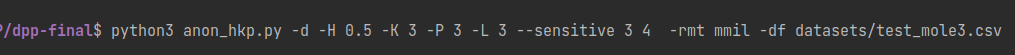
\includegraphics[scale=0.335]{test/prompt}
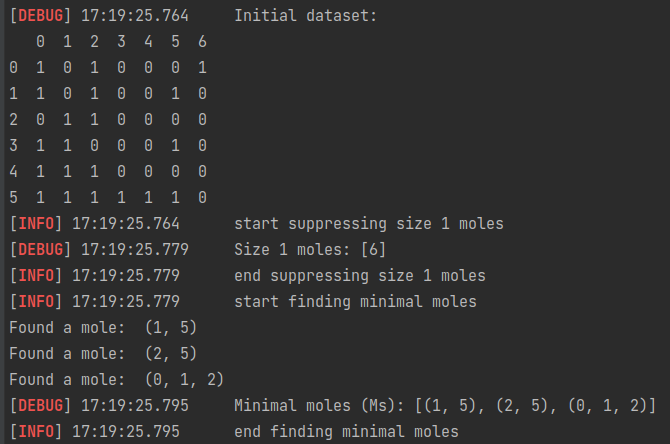
\includegraphics[scale=0.4]{test/part1}
\end{frame}
%--
\begin{frame}[fragile]
\frametitle{ }
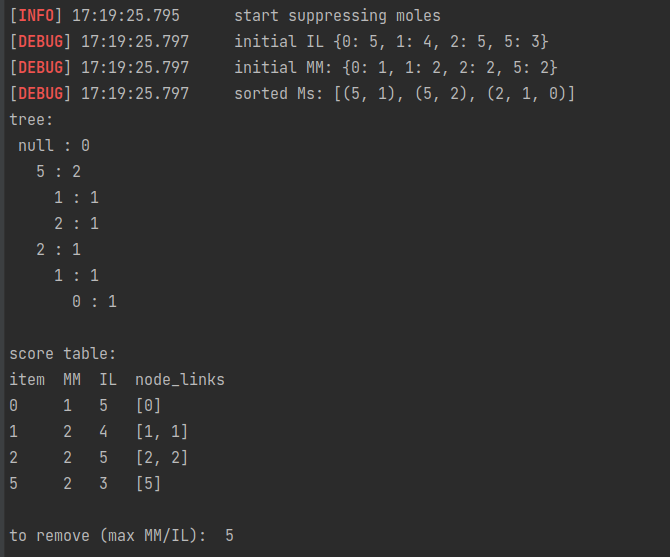
\includegraphics[scale=0.4]{test/part2_1}
\end{frame}
%--
\begin{frame}[fragile]
\frametitle{ }
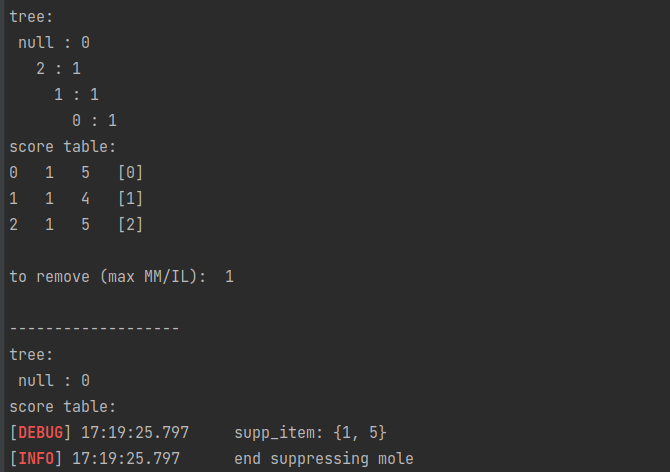
\includegraphics[scale=0.4]{test/part2_2}
\end{frame}
%--
\begin{frame}[fragile]
\frametitle{Result:}
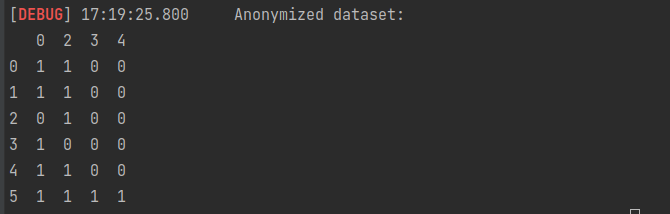
\includegraphics[scale=0.4]{test/result}

\vspace{0.5cm}
Dataset has been anonymized by removing columns: 1, 5, 6.\\
This represents the optimal solution: the choice max(MM/IL) for supp\_items finds the element e that ``appear" in most moles but also minimizes the information loss. 
\end{frame}
%--
\begin{frame}[fragile]
\frametitle{Experimental results}
To evaluate the efficiency of our algorithm we relied on the metrics presented on the paper:
\begin{itemize}
    \item We visualized the percentage of information loss after the anonymization (IL(supp\_item)/total information in D) at the variation of different parameters: \textbf{K}, \textbf{P} and \textbf{$\delta$}
    \item We compared different criteria for suppressing an item: \textbf{MM/IL}, \textbf{1/IL}, \textbf{remove\_all\_public}
\end{itemize}\\
\vspace{4mm}
We generated synthetic datasets and we evaluated the different performance results on the variation of some features: \textbf{density} of information and row/columns proportion.\\

\textbf{Note:} we choosed to plot the graphs for a single execusion with a fixed random seed to get consistent results.
\end{frame}
%--
\begin{frame}[fragile]
\frametitle{Results on dataset Connect: a failure}
Contrary to what is reported on the paper, the results on the dataset Connect did not show any benefits of using different elimination methods.\\
Connect size: $57'557x129$, k=100, p=l=5, h=0.4, $\delta$=40\%
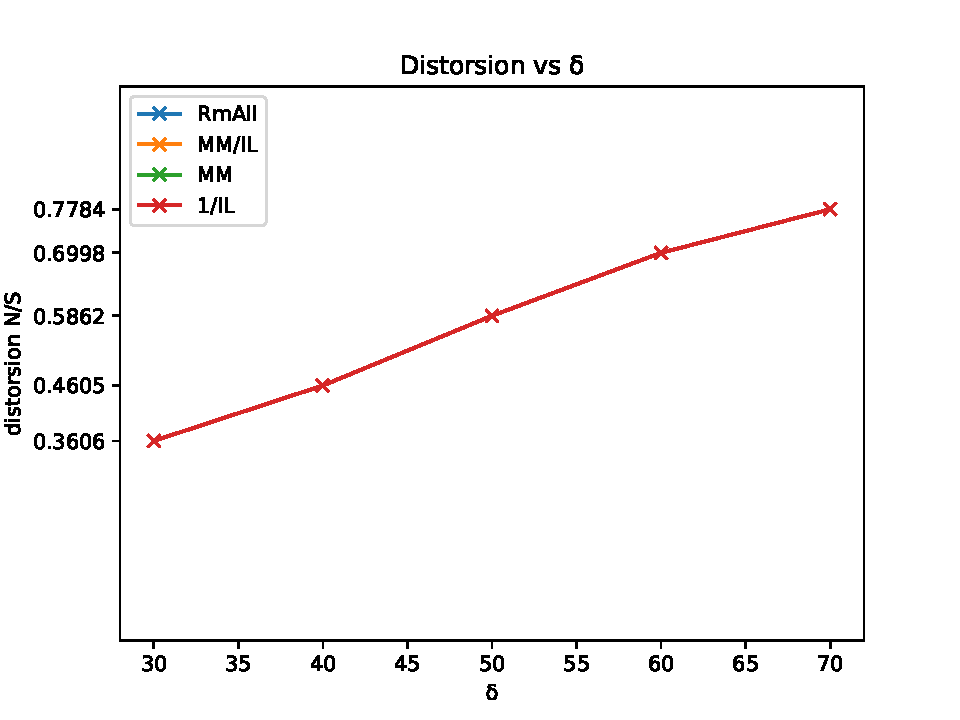
\includegraphics[scale=0.34]{img/plt_connect_delta_random}

\textbf{Why?} This behaviour may be caused by the distribution of the dataset: we noticed that support values of the columns are highly unbalanced, by random sampling the public items is then pretty easy to find a bad combination that brings up the number of the moles (p\_breach() only needs to find a max between many private items).
\end{frame}
%--
\begin{frame}[fragile]
\frametitle{Connect: Synthetic simulation}
Synthetic matrix size: $10000x20$, k=10, p=l=5, h=0.4, $\delta$=40\% \\
The density of the datset Connect is 0.3. We reproduced a more balanced, smaller synthetic version by keeping the same density and proportion row/columns:\\

\begin{figure}
    \begin{subfigure}[a]{0.32\linewidth}
        \centering
            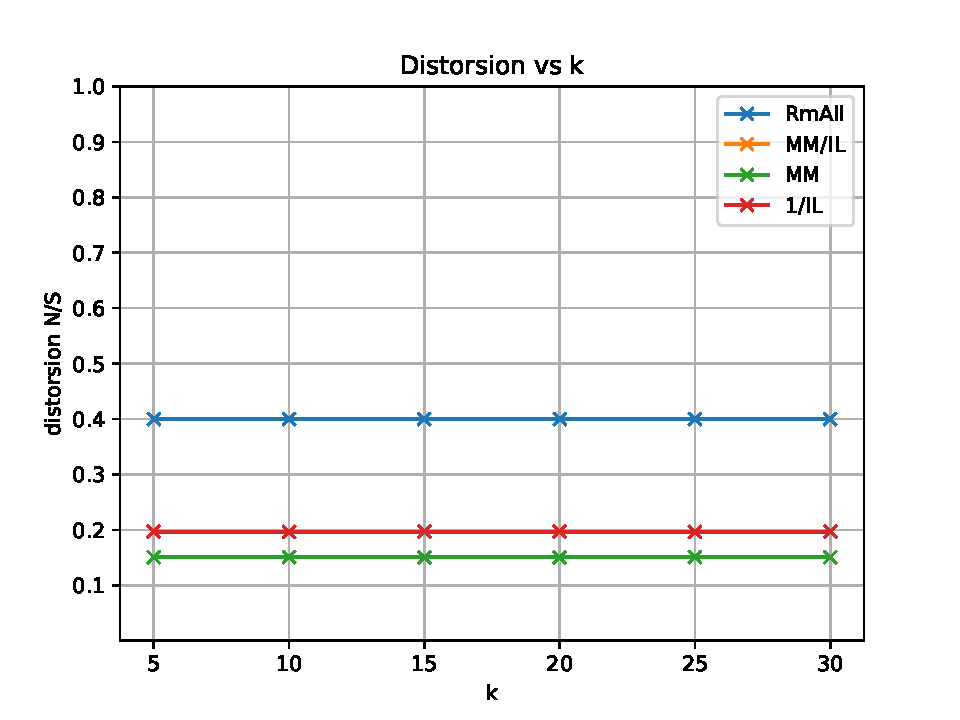
\includegraphics[width=\linewidth]{img/plt_ds_x10000_y20_d03_k_}
            \caption{K}\label{fig1a}
    \end{subfigure}
    \begin{subfigure}[b]{0.32\linewidth}
        \centering
            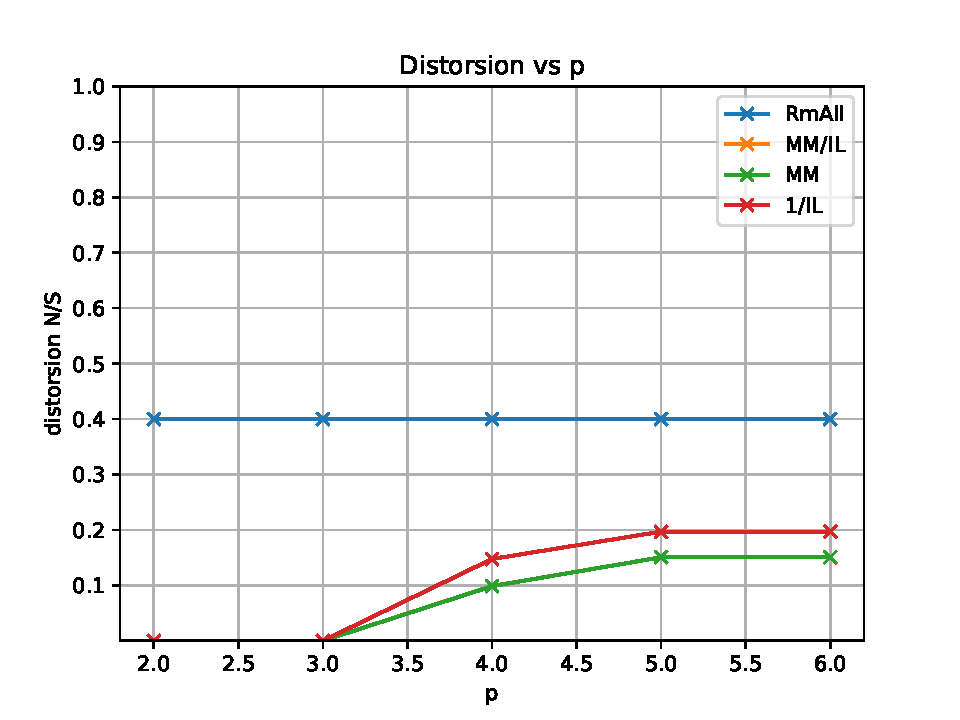
\includegraphics[width=\linewidth]{img/plt_ds_x10000_y20_d03_p_}
            \caption{P}\label{fig1a}
    \end{subfigure}
    \begin{subfigure}[c]{0.32\linewidth}
        \centering
            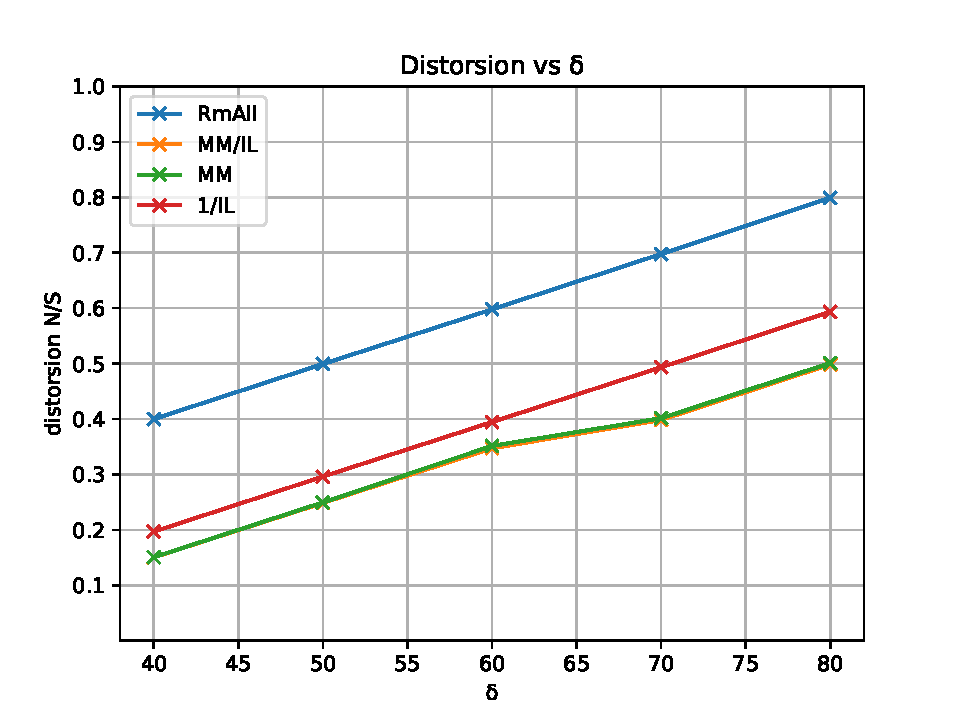
\includegraphics[width=\linewidth]{img/plt_ds_x10000_y20_d03_delta_}
            \caption{\delta}\label{fig1b}
    \end{subfigure}
\caption{Distorsion distribution for data density 0.3}
\end{figure}


\end{frame}
%--
\begin{frame}[fragile]
\frametitle{Results for different densities (same parameters):}
Density 0.1:
\begin{columns}[t]
\column{.33\textwidth}
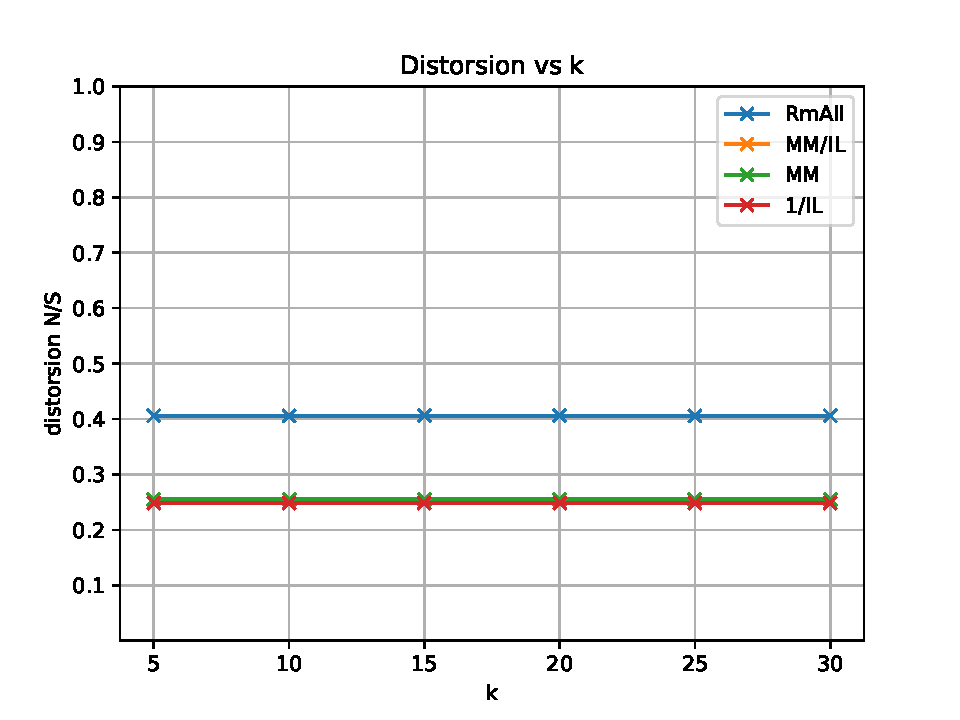
\includegraphics[scale=0.27]{img/plt_ds_x10000_y20_d01_k_}
\column{.33\textwidth}
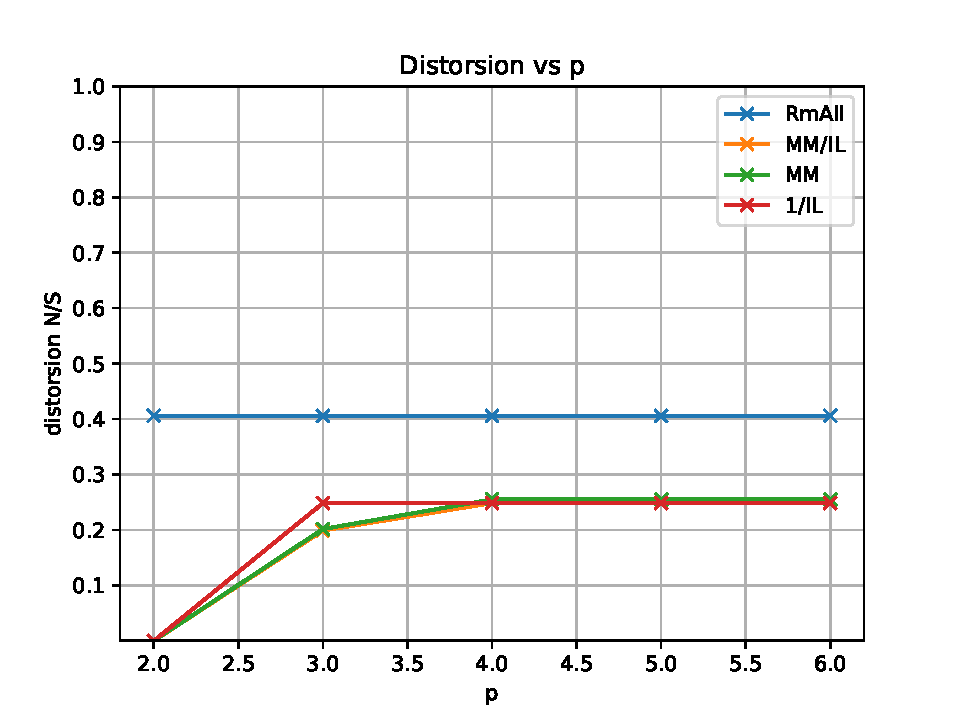
\includegraphics[scale=0.27]{img/plt_ds_x10000_y20_d01_p_}
\column{.33\textwidth}
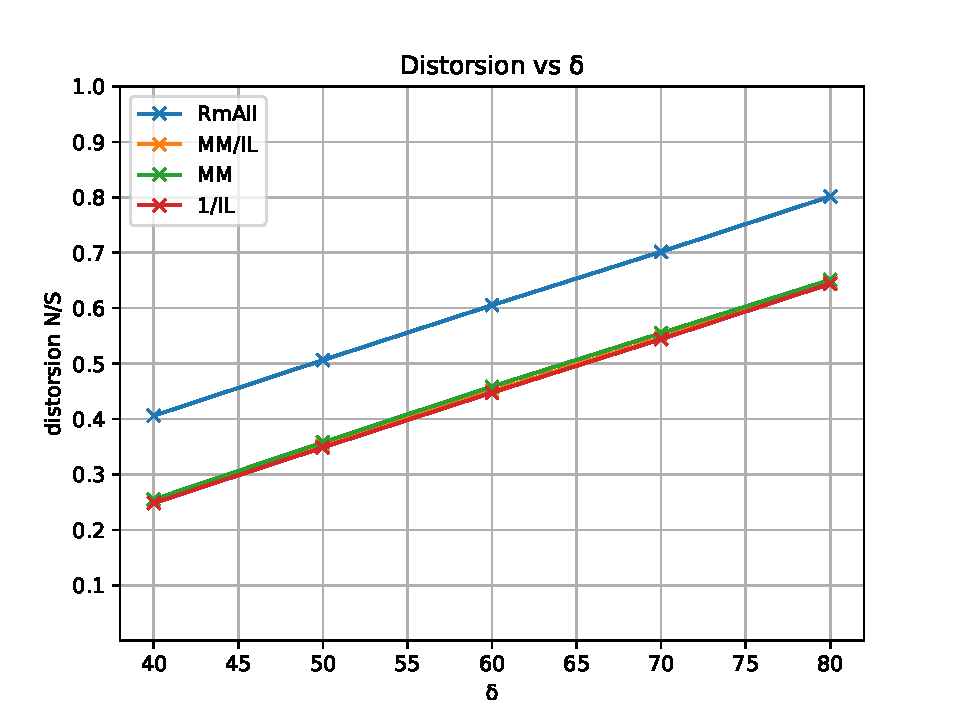
\includegraphics[scale=0.27]{img/plt_ds_x10000_y20_d01_delta_}
\end{columns}
Density 0.2
\begin{columns}[t]
\column{.33\textwidth}
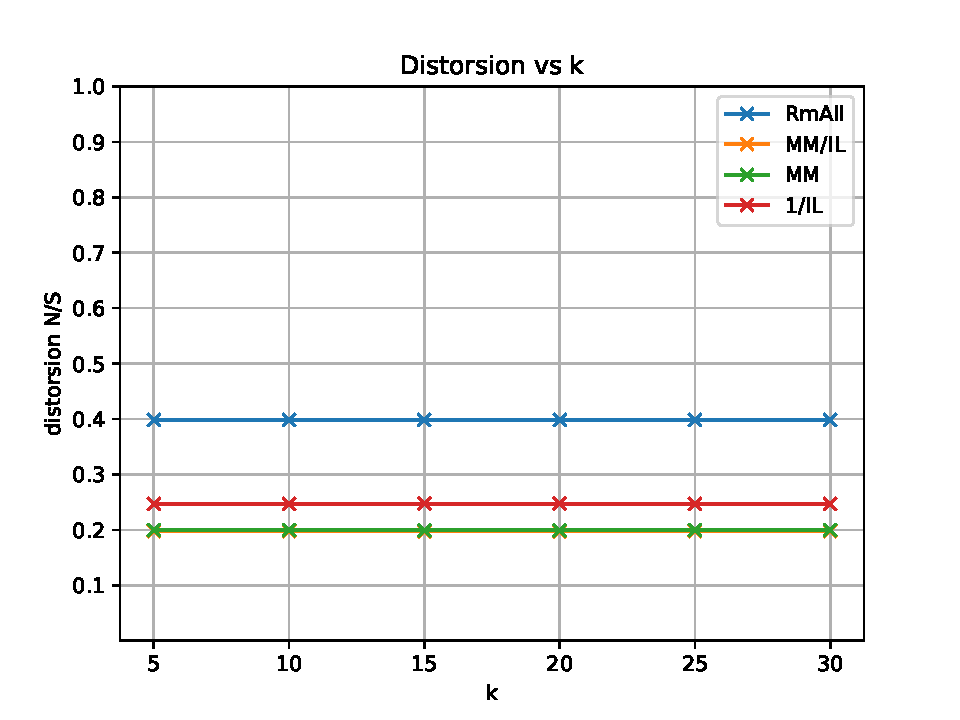
\includegraphics[scale=0.27]{img/plt_ds_x10000_y20_d02_k_}
\column{.33\textwidth}
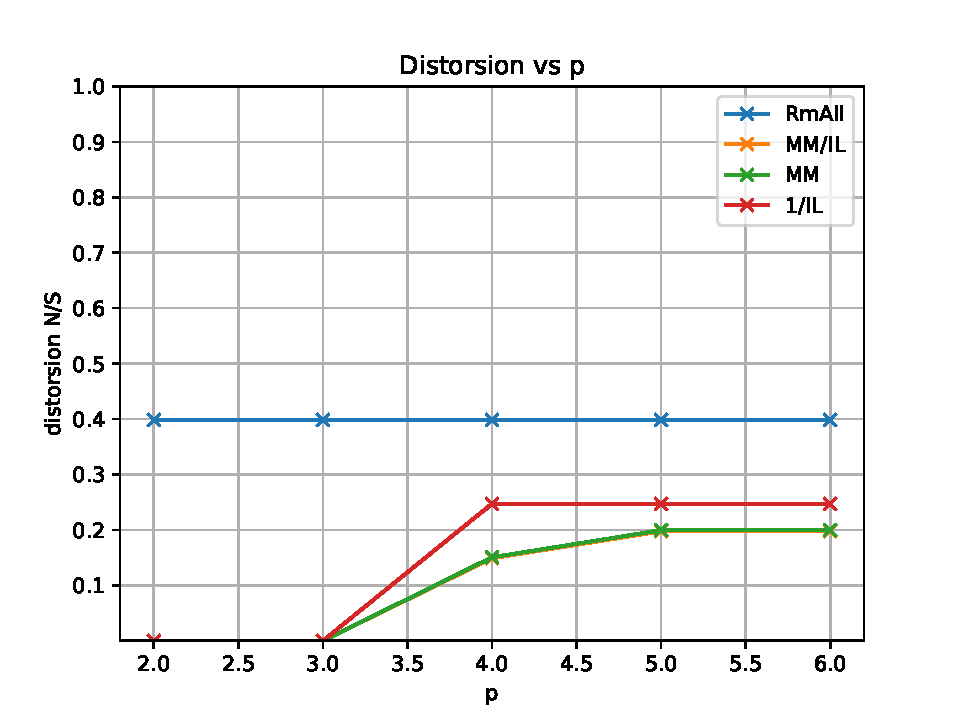
\includegraphics[scale=0.27]{img/plt_ds_x10000_y20_d02_p_}
\column{.33\textwidth}
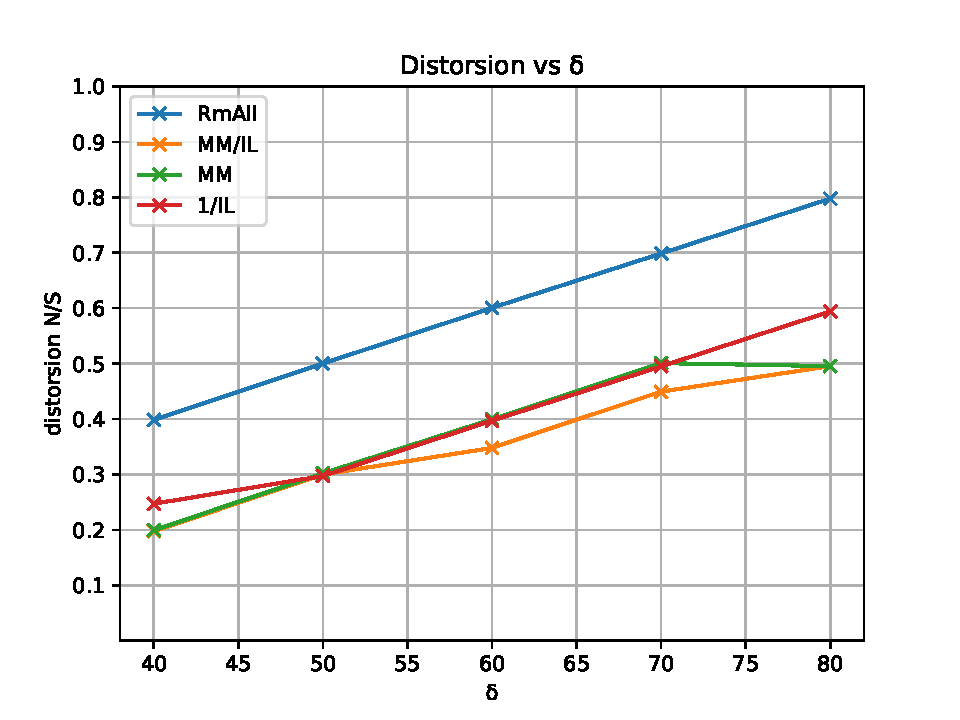
\includegraphics[scale=0.27]{img/plt_ds_x10000_y20_d02_delta_}
\end{columns}

\end{frame}
%--
\begin{frame}[fragile]
\frametitle{Conclusion}
\begin{itemize}
    \item It can be seen that the optimal elimination method is MM/IL since it takes in consideration both MM and IL
    \item The algorithm and the speed of our implementation are strongly affected by the characteristics of the input dataset: dimensions, density, information distribution
    \item An accurate tuning of all the parameters is needed to get a good result
\end{itemize}
\end{frame}
%--

\end{document}
